\documentclass[tikz,border=8pt]{standalone}
\usetikzlibrary{arrows.meta,positioning,calc}
\begin{document}
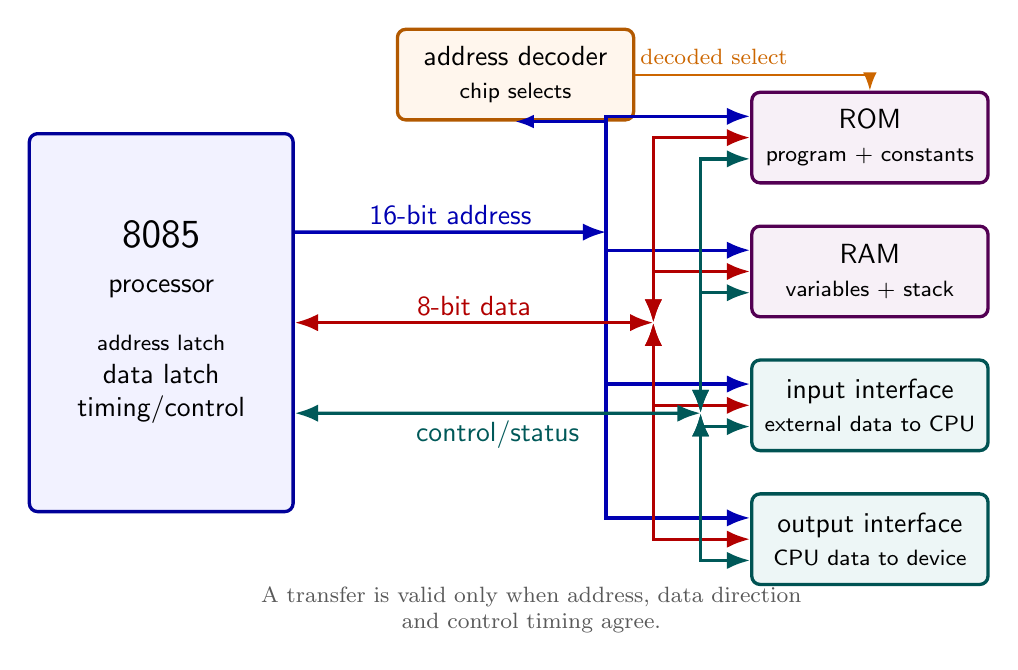
\begin{tikzpicture}[
  font=\sffamily,
  >=Latex,
  device/.style={draw=black!60,rounded corners=3pt,very thick,minimum width=3.0cm,minimum height=1.15cm,align=center,fill=black!2},
  memory/.style={device,draw=violet!65!black,fill=violet!6},
  io/.style={device,draw=teal!65!black,fill=teal!7}
]
  \node[device,minimum width=3.35cm,minimum height=4.8cm,fill=blue!5,draw=blue!60!black] (cpu) at (0,0) {\Large 8085\\[4pt]\normalsize processor\\[9pt]\footnotesize address latch\\data latch\\timing/control};
  \node[device,fill=orange!7,draw=orange!70!black] (dec) at (4.5,3.15) {address decoder\\\footnotesize chip selects};
  \node[memory] (rom) at (9,2.35) {ROM\\\footnotesize program + constants};
  \node[memory] (ram) at (9,.65) {RAM\\\footnotesize variables + stack};
  \node[io] (inp) at (9,-1.05) {input interface\\\footnotesize external data to CPU};
  \node[io] (out) at (9,-2.75) {output interface\\\footnotesize CPU data to device};

  \coordinate (atrunk) at (5.65,1.15);
  \coordinate (dtrunk) at (6.25,0);
  \coordinate (ctrunk) at (6.85,-1.15);

  \draw[->,very thick,blue!70!black] ([yshift=1.15cm]cpu.east) -- node[above,fill=white,inner sep=2pt]{16-bit address} (atrunk);
  \draw[->,very thick,blue!70!black] (atrunk) |- ([yshift=.27cm]rom.west);
  \draw[->,very thick,blue!70!black] (atrunk) |- ([yshift=.27cm]ram.west);
  \draw[->,very thick,blue!70!black] (atrunk) |- ([yshift=.27cm]inp.west);
  \draw[->,very thick,blue!70!black] (atrunk) |- ([yshift=.27cm]out.west);
  \draw[->,thick,blue!70!black] (atrunk) |- (dec.south);

  \draw[<->,very thick,red!70!black] (cpu.east) -- node[above,fill=white,inner sep=2pt]{8-bit data} (dtrunk);
  \draw[<->,very thick,red!70!black] (dtrunk) |- (rom.west);
  \draw[<->,very thick,red!70!black] (dtrunk) |- (ram.west);
  \draw[<->,very thick,red!70!black] (dtrunk) |- (inp.west);
  \draw[<->,very thick,red!70!black] (dtrunk) |- (out.west);

  \draw[<->,very thick,teal!70!black] ([yshift=-1.15cm]cpu.east) -- node[below,fill=white,inner sep=2pt]{control/status} (ctrunk);
  \draw[<->,very thick,teal!70!black] (ctrunk) |- ([yshift=-.27cm]rom.west);
  \draw[<->,very thick,teal!70!black] (ctrunk) |- ([yshift=-.27cm]ram.west);
  \draw[<->,very thick,teal!70!black] (ctrunk) |- ([yshift=-.27cm]inp.west);
  \draw[<->,very thick,teal!70!black] (ctrunk) |- ([yshift=-.27cm]out.west);

  \draw[->,thick,orange!80!black] (dec.east) -- node[above,font=\footnotesize]{decoded select} ++(2.0,0) -| (rom.north);
  \node[font=\footnotesize,text=black!65,align=center] at (4.7,-3.65) {A transfer is valid only when address, data direction\\and control timing agree.};
\end{tikzpicture}
\end{document}
